%%%%%%%%%%%%%%%%%%%%%%%%%%%%%%%%%%%%%%%%%%%%%%%%
%%   TEMPLATE MAIN FILE                       %%
%%%%%%%%%%%%%%%%%%%%%%%%%%%%%%%%%%%%%%%%%%%%%%%%

\documentclass[10pt,reqno,sumlimits]{amsart}
\usepackage{amssymb}
\usepackage{epsfig}
\usepackage{multirow}
\usepackage{graphics}
\usepackage{graphicx}
\usepackage{subfigure}
\usepackage{url}
%\textwidth 6.2in
%\oddsidemargin.20in
%\evensidemargin.35in
%%\lineskip 1in
%%\baselineskip.55cm

% Read in specially defined commands
% Change margins and baselinestretch in draft mode
\def\draft{
% make margins smaller
\addtolength{\oddsidemargin}{-0.5in}
\addtolength{\topmargin}{-0.65in}
\addtolength{\textheight}{1in}
\addtolength{\textwidth}{1.5in}
% A more reasonable baselinestretch, is still nearly doublespaced.
\def\baselinestretch{1.4}
}

%\vfuzz2pt % Don't report over-full v-boxes if over-edge is small
%\hfuzz2pt % Don't report over-full h-boxes if over-edge is small

%%%%%%%%%%%%%%%%%%%%%%%%%%%%%%%%%%%%%%%%%%%%%%%%%%%%%%%%
%%              Theorems                               %
%%%%%%%%%%%%%%%%%%%%%%%%%%%%%%%%%%%%%%%%%%%%%%%%%%%%%%%%
\theoremstyle{plain}
\newtheorem{theorem}{Theorem}
\newtheorem{corollary}[theorem]{Corollary}
\newtheorem{lemma}[theorem]{Lemma}
\newtheorem{proposition}[theorem]{Proposition}
\newtheorem{conjecture}[theorem]{Conjecture}

\theoremstyle{definition}
\newtheorem{remark}[theorem]{Remark}
\newtheorem{definition}[theorem]{Definition}
\newtheorem{example}[theorem]{Example}
\newtheorem{notation}{Notation}

%%%%%%%%%%%%%%%%%%%%%%%%%%%%%%%%%%%%%%%%%%%%%%%%%%%%%%%%
%%      Definitions and Commands                       %
%%%%%%%%%%%%%%%%%%%%%%%%%%%%%%%%%%%%%%%%%%%%%%%%%%%%%%%%
\newcommand{\A}{{\mathbb A}}
\newcommand{\R}{{\mathbb R}}
\newcommand{\Q}{{\mathbb Q}}
\newcommand{\C}{{\mathbb C}}
\newcommand{\D}{{\mathbb D}}
\newcommand{\Z}{{\mathbb Z}}
\newcommand{\h}{{\mathbb H}}
\newcommand{\CP}{{\mathbb C}{\mathbb P}}
\newcommand{\I}{{\mathbb I}}
\newcommand{\N}{{\mathbb N}}
%
\newcommand{\calA}{{\mathcal A}}
\newcommand{\calB}{{\mathcal B}}
\newcommand{\calC}{{\mathcal C}}
\newcommand{\calD}{{\mathcal D}}
\newcommand{\calE}{{\mathcal E}}
\newcommand{\calF}{{\mathcal F}}
\newcommand{\calG}{{\mathcal G}}
\newcommand{\calH}{{\mathcal H}}
\newcommand{\calI}{{\mathcal I}}
\newcommand{\calK}{{\mathcal K}}
\newcommand{\calM}{{\mathcal M}}
\newcommand{\calO}{{\mathcal O}}
\newcommand{\calP}{{\mathcal P}}
\newcommand{\calR}{{\mathcal R}}
\newcommand{\calS}{{\mathcal S}}
\newcommand{\calL}{{\mathcal L}}
\newcommand{\calX}{{\mathcal X}}
\newcommand{\calU}{{\mathcal U}}
\newcommand{\calV}{{\mathcal V}}
\newcommand{\calZ}{{\mathcal Z}}
%
\newcommand{\ggoth}{{\mathfrak  g}}
\newcommand{\ugoth}{{\mathfrak  u}}
\newcommand{\hgoth}{{\mathfrak  h}}
%%
\newcommand{\1}{{\bf 1}}
\newcommand{\acts}{{\circlearrowright}}
\newcommand{\ex}[1]{{e^{#1}}}
\newcommand{\dd}[2]{\frac{\partial #1}{\partial #2}}
\newcommand{\iso}{\stackrel{\simeq}{\longrightarrow}}
\newcommand{\spinc}{$\text{spin}^c$}
\newcommand{\Dirac}{\not\!\!D}
\newcommand{\inc}{\hookrightarrow}
%%
\newcommand{\Aut}{\operatorname{Aut}}
\newcommand{\Hom}{\operatorname{Hom}}
\newcommand{\Hor}{\operatorname{Hor}}
\newcommand{\Ext}{\operatorname{Ext}}
\newcommand{\End}{\operatorname{End}}
\newcommand{\Map}{\operatorname{Map}}
\newcommand{\Diff}{\operatorname{Diff}}
\newcommand{\Tr}{\operatorname{Tr}}
\newcommand{\Lie}{\operatorname{Lie}}
\newcommand{\ad}{{\operatorname{ad\,}}}
\newcommand{\sign}{{\operatorname{sign}}}
\newcommand{\grad}{{\operatorname{grad}}}
\newcommand{\coker}{{\operatorname{coker}}}
\newcommand{\dett}{{\operatorname{det}}}
\newcommand{\ch}{{\operatorname{ch}}}
\newcommand{\rk}{{\operatorname{rk}}}
\newcommand{\maxx}{{\operatorname{max}}}
\newcommand{\minn}{{\operatorname{min}}}
\newcommand{\id}{{\operatorname{id}}}
\newcommand{\ind}{{\operatorname{ind}}}
\newcommand{\Ind}{{\operatorname{Ind}}}
\newcommand{\spann}{{\operatorname{span}}}
\newcommand{\Spin}{{\operatorname{Spin}}}
\newcommand{\Pin}{{\operatorname{Pin}}}
\newcommand{\im}{{\operatorname{Im}}}
\renewcommand{\Im}{{\operatorname{Im}}}
\newcommand{\dimm}{{\operatorname{dim}}}
\newcommand{\cl}{{\operatorname{cl}}}
%%
\newcommand{\tM}{{\tilde{M}}}
\newcommand{\tC}{{\tilde{C}}}
\newcommand{\tE}{{\tilde{E}}}
\newcommand{\tF}{{\tilde{F}}}
\newcommand{\talpha}{{\tilde{\alpha}}}
%%
\newcommand{\zbar}{\overline{z}}
\newcommand{\wbar}{\overline{w}}
\newcommand{\phibar}{\overline{\phi}}
\newcommand{\psibar}{\overline{\psi}}
\newcommand{\Bbar}{\overline{B}}
\newcommand{\Cbar}{\overline{C}}
\newcommand{\inv}{^{-1}}
%%      
\newcommand{\rb}[1]{\raisebox{0pt}[0pt][0pt]{#1}}
\newsavebox{\savepar}
\newenvironment{boxit}{\begin{lrbox}{\savepar}\begin{minipage}[b]{.5in}}
{\end{minipage}\end{lrbox}\fbox{\usebox{\savepar}}}
%%\newcommand{\ip}[1]{\langle\! #1 \! \rangle}
\newcommand{\ip}[1]{\langle #1 \rangle}
\newcommand{\norm}[1]{\| #1 \|}
%
%\newcommand{\remark}{{\tt ?}\marginpar{\Large\centering ?}}
\newcommand{\rremark}{\marginpar{\Large\centering ?}}
\newcommand{\Remark}[1]{\textsc{\tiny{[#1]}}\rremark}
\newcommand{\todo}{\textsc{Todo!}\marginpar{\Large\centering !}}
%
\numberwithin{equation}{section}
\renewcommand{\theequation}{{\thesection{.}}\arabic{equation}}
\newcounter{dummy}
%
%%%%%%%%%%%%%%%%%%%%%%%%%%%%%%%%%%%%%%%%%%%%%%%%%%%%%%%
\begin{document}

\title[Assignment 2]{The Plot Thickens}
\author{Joe Smith}


%\begin{abstract}
%The abstract
%\end{abstract}

\maketitle

%\tableofcontents

%%%%%%%%%%%%%%%%%%%%%%%%%%%%%%%%%%%%%%%%%%%%%%%%%%%%%%%

\section {Closed Union}
Prove that the class of regular languages is closed under the union ($\cup$) operation. (Hint: Use proof by construction.)

A collection of objects is closed under an operation if applying the operation to members of the collection returns an object in the collection.

Alright, I think I got this one. Take a regular language, $R_1$. Because it is regular, there is a Regular Expression, $r_1$, that describes it. Now take a second regular language, $R_2$, which also has a regular expression that describes it, $r_2$.

Then the union of $R_1$ and $R_2$ is $L$. Language $L$ is described by the regex $r_1 \cup r_2$, which by definition of a regular expression is regular. Thus, since there is a regex that describes $L$, it is regular.

\section{...now has two problems}
Provide the regular expression that corresponds to each of the following language descriptions. Assume that $\Sigma$ is \{0, 1\}:

\begin{enumerate}
\item \{$w|w$ has exactly a single 1\}

\hspace{0.5in} $0^*\ \cdot\ \{1\}\ \cdot\ 0^*$

\item \{$w|w$ contains the string 001 as a substring\}

\hspace{0.5in} $\Sigma^*\ \cdot\ \{001\}\ \cdot\ \Sigma^*$

\item \{$w|w$ is a string of even length\}

\hspace{0.5in} $ (\{0,1\} \cdot \{0,1\})^*$

\item \{$w|w$ starts and ends with the same symbol\}

\hspace{0.5in} $ a\ \in\ \Sigma,\ a \cdot \Sigma^* \cdot a  $

\end{enumerate}

\section{Regex to NFA}
Convert the regular expression $(a \cup b)^*$ to a nondeterministic finite state automaton. Note that you do not have to draw the NFA if you do not wish to do so. You may provide the mathematical specification $M = (Q, \Sigma, \delta, q_0 , F )$. For $\delta$ you may provide a table of the transitions.

\begin{figure}[htbp]
\centerline{
    \mbox{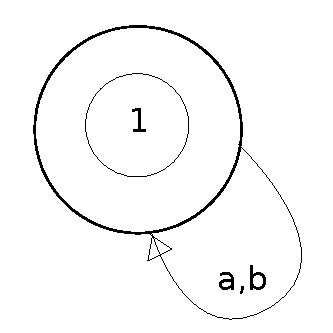
\includegraphics[width=1.5in]{algorithms2_3.pdf}}
  }
  \caption{$(a \cup b)^*$}
  \label{fig:fit}
\end{figure}

\hspace{0.5in} This seems almost deceptively simple, but it would appear that this is a rather simple Regex to model. $M = (Q, \Sigma, \delta, q_0 , F )$, where:

\vspace{0.2in}
$ Q = 1$

$\Sigma = a,\ b$

$\delta = \{1\}_a \rightarrow \{1\}, \{1\}_b \rightarrow \{1\}$

$q_0 = 1$

$F = 1$.
\vspace{0.2in}

\section{Pump it up}
Using the pumping lemma prove that $F = \{ww|w\ \in\ \{0, 1\}\ \}$ is nonregular.

To prove $F$ is nonregular, let's assume it is regular, with pumping length $P$.

There must exist a string:

\hspace{0.3in}$S = x y z$ for $i \geq 0$ such that $x$ is a $w$ and $y$ is a $w$.

Then say $P$ is two. If you pump $y$, you will get:

\hspace{0.3in}$xyyy$, where those equal $wwww$, which is no longer part of the language.



\end{document}

%%%%%%%%%%%%%%%%%%%%%%%%%%%%%%%%%%%%%%%%%%%%%%%%%%%%%%%

%%% Local Variables: 
%%% mode: latex
%%% TeX-master: "main"
%%% End: 

